\documentclass{book}

\usepackage[]{graphicx}
\usepackage[]{float}

\title{Design Document}
\author{Jens Henninger \and Daniel Maier \and Paul Fink \and Florian Jennewein}
\date{\today}


\begin{document}
\frontmatter
\maketitle
\tableofcontents
\mainmatter
\part{Architectural Design}

\chapter{Introduction}
This architectural document describes the architecture of the desired system 
"Sojabohne" from different perspectives and in different levels of detail. 
All references to requirements are based on the system requirements of our requirements-document from 26.11.2015\footnote{https://moodle.uni-mainz.de/pluginfile.php/33185/assignsubmission\_file/submission\_files/8942/Abgabe\_Review\_Document.tar.gz}.
\chapter{External Layer}
Because there is no connection between our system and other ones,
 Sojabohne is set in a standalone-context(cf.Figure 2.1). 
\begin{figure}[H]
\centering
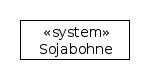
\includegraphics[width=3cm]{Diagrams/Context_Model.jpg}
\caption{Our system in standalone context :)}
\label{Fig. 1}
\end{figure}
\chapter{Structural Layer}
\section{Basic}
Obviously the most basic systemstructure is based on the Client-Server Pattern.
That's because in this pattern, the server provides services, in our case mainly
the execution of data mining and machine learning algorithms on a user uploaded data.
An user shall be able to access the result and the data itself from all over the
world(if he has the required rights to do so) via the web application(cf. NFR017.0/NFR005.0). 
So we use the client-server-pattern, where the web application is the client and the server
is the system, who executes the algorithms inclusive the database(cf. Fig. 3.1).
\begin{figure}[H]
\centering
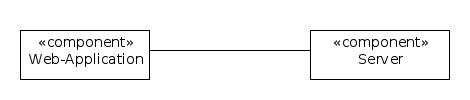
\includegraphics[width=9cm]{Diagrams/Client-Server.jpg}
\caption{Web-application as client; with the server.}
\label{Fig. 2}
\end{figure}
\section{Client} 
For the client structure we use the layer-pattern, to  ensure the requested modularity (cf. NFR026.0).
So every layer can be changed, updated or replaced without any complications as long as
 the new components are based on the right interfaces.\\
We split our client in three sections: the presentation-, the logic- and the data section.\\
The highest level is the presentation; the only part of the web-application, a normal user
can interact with. There are three surfaces needed for the whole presentation: 
the user-(for FR005.0, Fr009 1./2.), the upload/download(for the rest of FR009) surface for everything
regarding up- and downloding data and the visulalization-(FR009 3. without the up- and downloading)
for the result and data representation and . The posibility to switch between this surfaces is 
representated by the connections between them(cf. Fig 3.2).\\
The components in the logic section are used to control the computer operations standing behind the
surfaces.\\
The only component in the data section is used for communication/connection between the web- application
and the server, because there's no data stored or processed in the web-app itself.\\
In our case we have a clean seperation between our layers, because each level can only interact only
with neighbouring levels, where each communication is triggered by the highest level.
\begin{figure}[H]
\centering
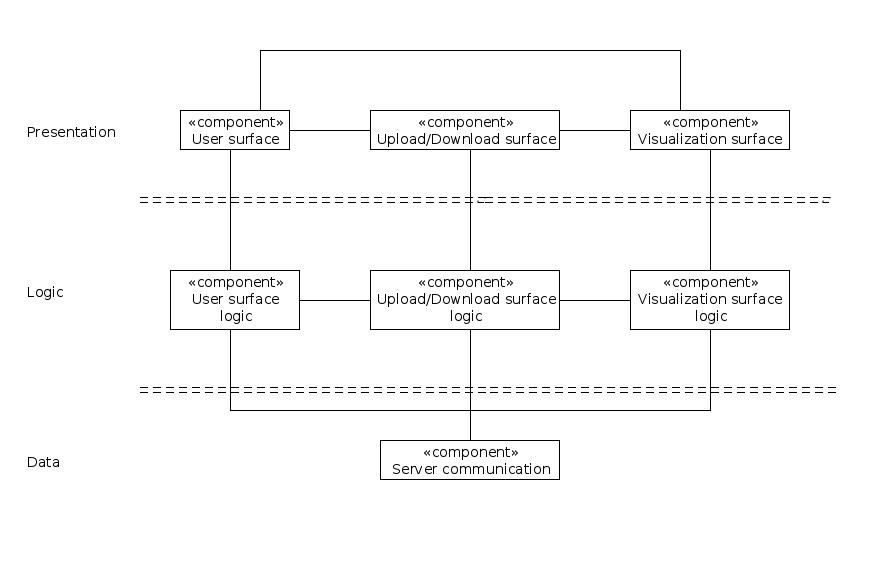
\includegraphics[width=16cm]{Diagrams/Overview.jpg}
\caption{Client overview}
\label{Fig. 3}
\end{figure}
Next we look at the first two sections in greater detail. First the user-perspective and its logical component:\\ This perspective can be divided into two parts.\\ First a registration/login component(cf. FR005) and second an administrative component (e.g. changing permissions on data packages; cf. FR009 1./2.). To realize those components we used model-view-controller-pattern, which has three parts: model, view and controller. In our case this means for example that when a user tries to login to our system he/she enters the data into the login-view, which informs the login-controller. The controller now communicates with the logic level, which contains the login-model. The model sends a request to the data level and through it to the database to check the given information for its correctness. After receiving that information the model informs the controller, which relays the  
it in readable form for the user to the login-view. That's in our opinion the most effective way to ensure user permissions(by checking his given data (e.g. password);cf. FR010-FR013; Fig. 3.3).
\begin{figure}[H]
\centering
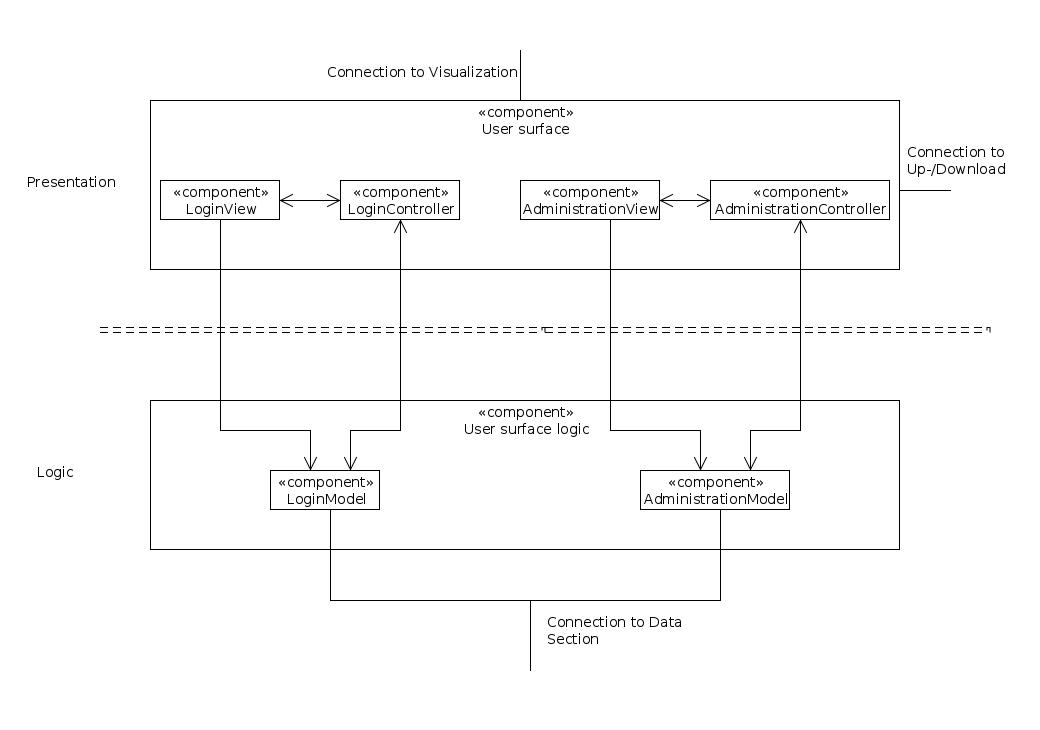
\includegraphics[width=16cm]{Diagrams/User_surface.jpg}
\caption{User surface zoom}
\label{Fig. 4}
\end{figure}
Next to the user perspective we have the up- and download perspective. Which we can obviously divide into an up- and a download component. We used the model-view-controller pattern portray these components(for permission checking and modularity; cf. FR010-FR013; Fig. 3.4). Additionally there is a converter, which turns the output into a user chosen format (e.g. pdf).
\begin{figure}[H]
\centering
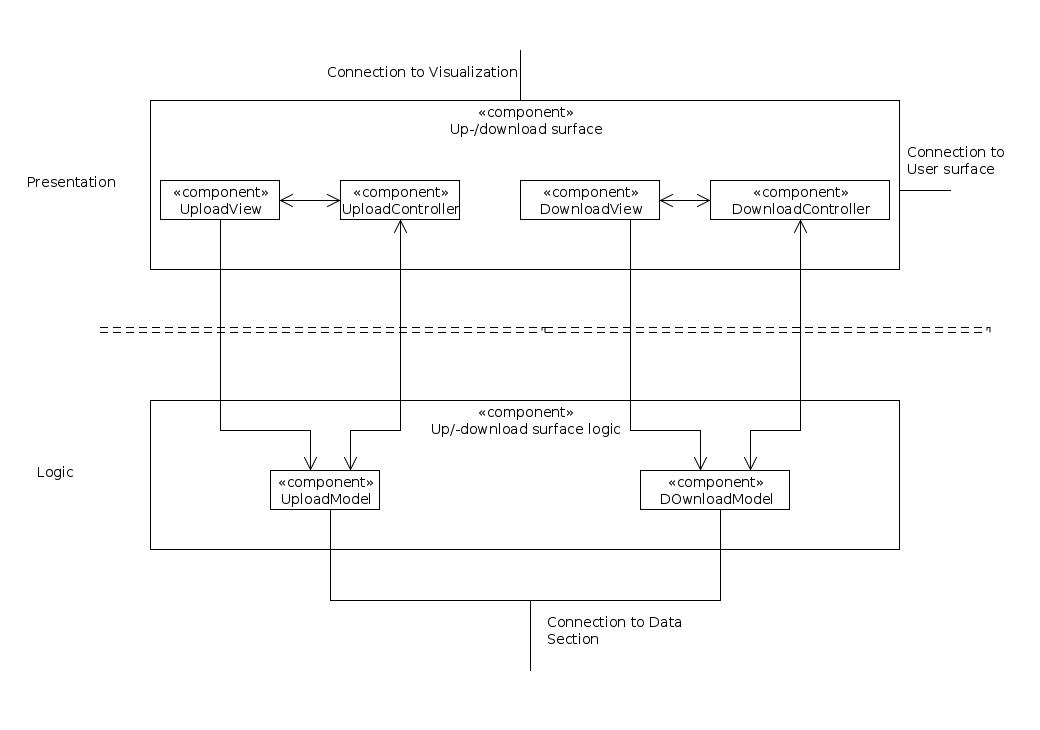
\includegraphics[width=16cm]{Diagrams/load_surface.jpg}
\caption{Up-/download surface zoom}
\label{Fig. 5}
\end{figure}
For the same reasons we used this pattern for the visualization surface. Here, in our opinion is the most important advantage the modularity of result representation (cf. Fig. 3.5).
\begin{figure}[H]
\centering
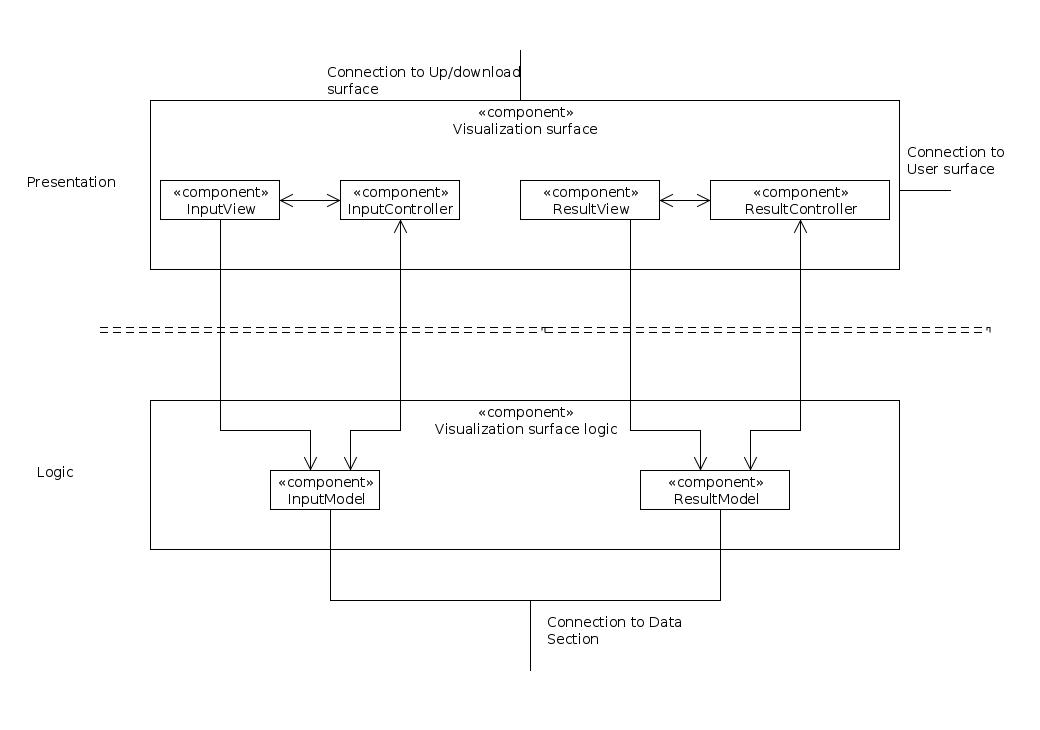
\includegraphics[width=16cm]{Diagrams/vis_surface.jpg}
\caption{Visualization surface zoom}
\label{Fig. 6}
\end{figure}
\subsection{Server}
For the server we used the pattern layer again. The first level is the web-application-interface, which realizes the communication between server and web-application. The second level is the request-form level. Any kind of request to the server uses forms, for example the login uses a login form or to upload test data, we have an upload-data form. This level checks these forms for their correctness. Below that we have the processing level, which performs the given request(including the rights management). Lastly we have the database itself, which saves all given and calculated data(cf. Fig 3.6).
\begin{figure}[H]
\centering
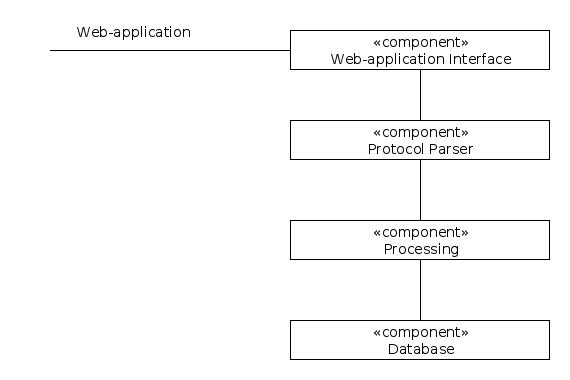
\includegraphics[width=10cm]{Diagrams/server.jpg}
\caption{Server view}
\label{Fig. 7}
\end{figure}
For adding new algorithms and general extensibility we used a combination of the microkernel and the reflection pattern. The microkernel pattern is the only pattern that allows adding new functionality to the system and guaranties the portability to other systems. The reflection pattern allows us to get the metadata of the algorithm.
This way the algorithm just need to implement an interface which informs that what information the system needs. It does not need to know how the system later uses algorithm or how the system works in general. The other way around its is easy for the system to read what kind of parameters the algorithm needs to work properly (cf. Fig.3.7).
\begin{figure}[H]
\centering
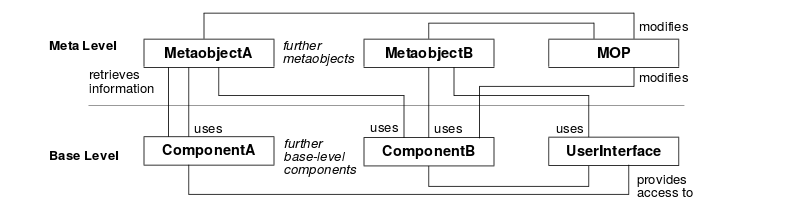
\includegraphics[width=15cm]{Diagrams/reflection.png}
\caption{The reflection pattern based on http://wiki.ifs.hsr.ch/APF/files/Reflection.pdf}
\label{Fig. 8}
\end{figure}
\chapter{Unused Patterns}
\textbf{Repository-Pattern:} Not used because we only have the web-application and not mobile apps or desktop clients. Therefore the server can be adjusted towards the web-application.\\
\textbf{Broker-Pattern:} Our system runs only on one server and not multiple.
\chapter{Interaction Layer}
The following section attends to the interaction between the different aleready mentioned system components in different scenarios. The main task is the visualization of the data exchange with sequence-diagrams; without an exact definition of the called methods.
\subsection{Login:}
Client-view:
\begin{figure}[H]
\centering
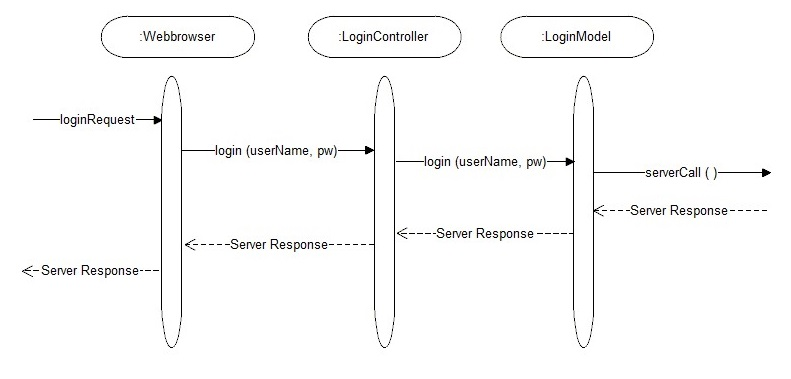
\includegraphics[width=15cm]{Diagrams/Login WebSicht.jpg}
\caption{Client-view of a login interaction}
\label{Fig. 9}
\end{figure}
Server-view:
\begin{figure}[H]
\centering
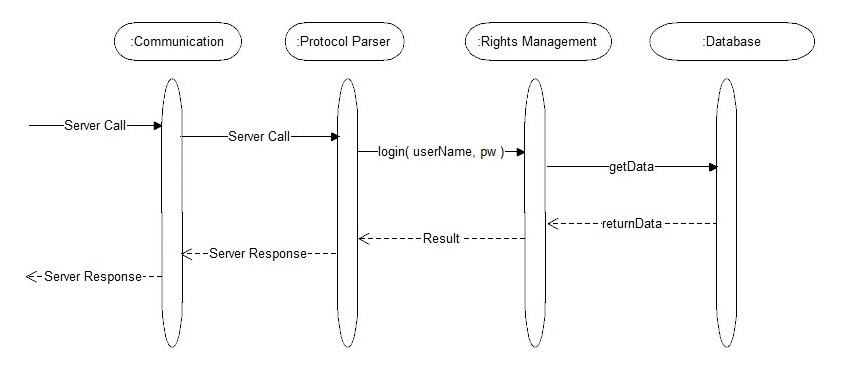
\includegraphics[width=15cm]{Diagrams/Login ServerSicht.jpg}
\caption{Server-view of a login interaction}
\label{Fig. 10}
\end{figure}
\subsection{Testing:}
Client-view:
\begin{figure}[H]
\centering
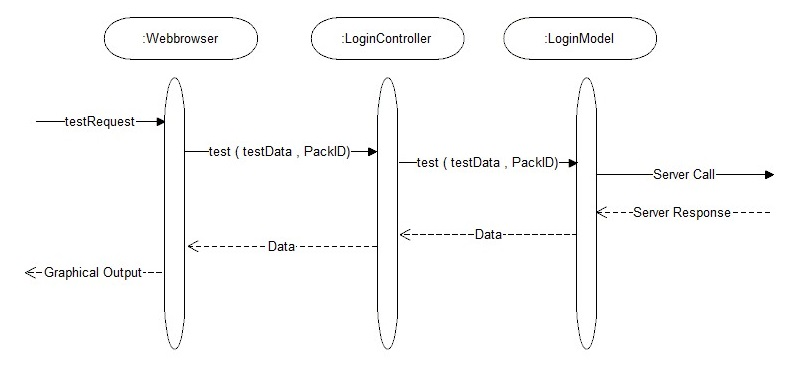
\includegraphics[width=15cm]{Diagrams/test WebSicht.jpg}
\caption{Client-view of a test interaction}
\label{Fig. 11}
\end{figure}
Server-view:
\begin{figure}[H]
\centering
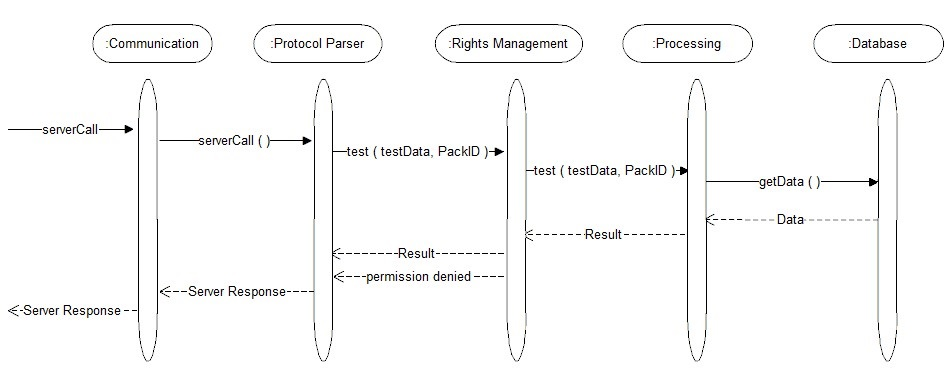
\includegraphics[width=15cm]{Diagrams/test ServerSicht.jpg}
\caption{Server-view of a test interaction}
\label{Fig. 12}
\end{figure}
\subsection{Uploading data:}
Client-view:
\begin{figure}[H]
\centering
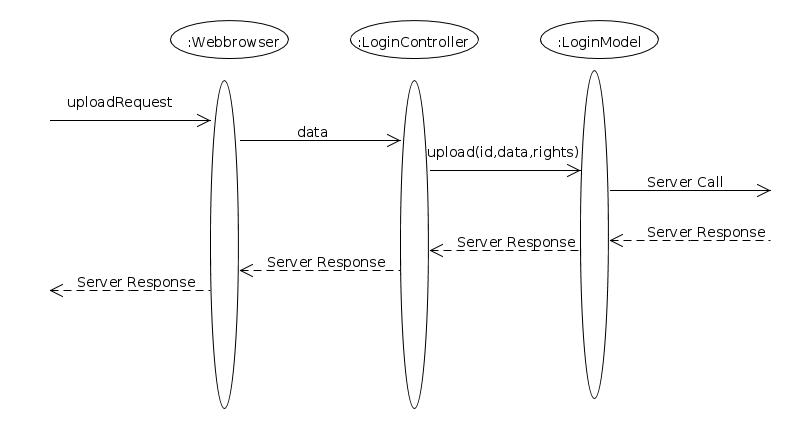
\includegraphics[width=15cm]{Diagrams/upload WebSicht.jpg}
\caption{Client-view of a upload interaction}
\label{Fig. 13}
\end{figure}
Server-view:
\begin{figure}[H]
\centering
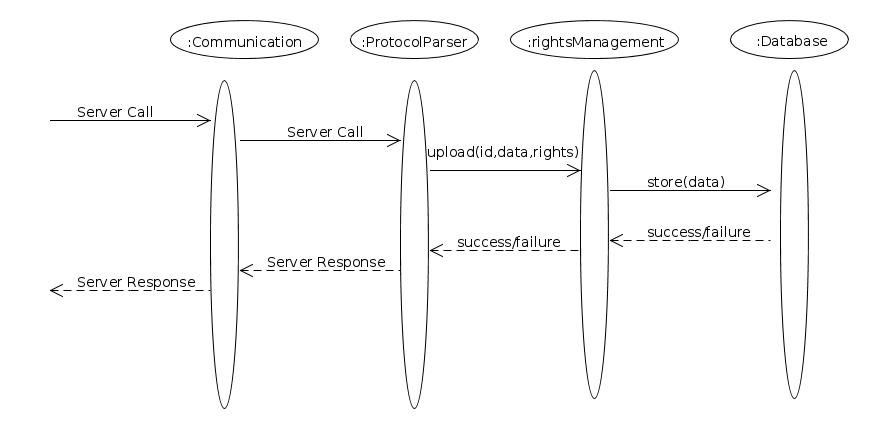
\includegraphics[width=15cm]{Diagrams/upload ServerSicht.jpg}
\caption{Server-view of a upload interaction}
\label{Fig. 14}
\end{figure}
\end{document}

%%% Local Variables:
%%% mode: latex
%%% TeX-master: t
%%% End:
